\chapter{Cấu trúc dữ liệu blockchain}

\section{Cây Merke}

%
%Biểu đồ trên miêu tả hình dạng của một một cây Merkle. Trong một cây Merkle, mỗi nút không-phải-lá là mã băm của giá trị của nút cây con của chúng.
%
%Nút lá: Nút là là những nút ở hàng thấp nhất của câu. Trong biểu đồ trên, các nút lá sẽ là L1, L2, L3 và L4.

Trong mật mã học và khoa học máy tính, một cây hash hoặc cây Merkle là một cây mà trong đó mỗi nút lá đều được gắn với mã băm của một khối dữ liệu và mọi nút không-phải-nút-lá được gắn với mã băm mật mã của con nó. Cây hash cho phép việc chứng thực hiệu và an toàn nội dung của các cấu trúc dữ liệu lớn.

\begin{figure}[h]
	\centering
	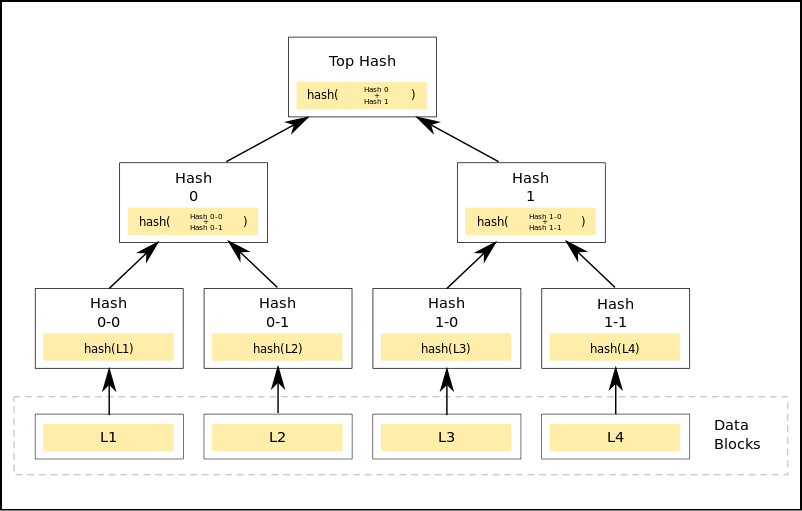
\includegraphics[width=0.9\textwidth]{merkleTree}
	\caption{Một ví dụ của cây hash nhị phân. Nguồn: Wikipedia}
	
\end{figure}

\section{Cấu trúc dữ liệu Blockchain}
Blockchain là một danh sách liên kết chứa dữ liệu và một con trỏ hash chỉ đến block trước nó, tạo thành một chuỗi (chain).

\begin{figure}[h]
	\centering
	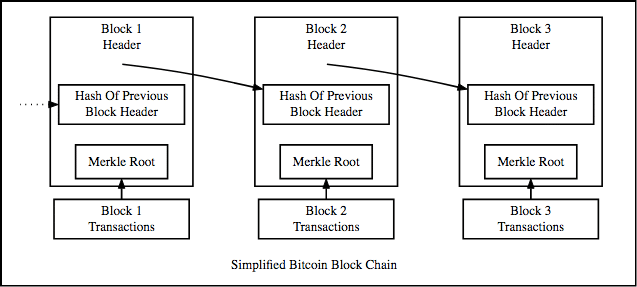
\includegraphics[width=0.9\textwidth]{blockchainStruct}
	\caption{Minh họa cấu trúc dữ liệu blockchain}
	
\end{figure}

Con trỏ hash giống như một con trỏ thường, nhưng chỉ chứa điạ chỉ của block trước nó, cũng như mã băm của dữ liệu bên trong block đó (block trước nó).

\begin{figure}[h]
	\centering
	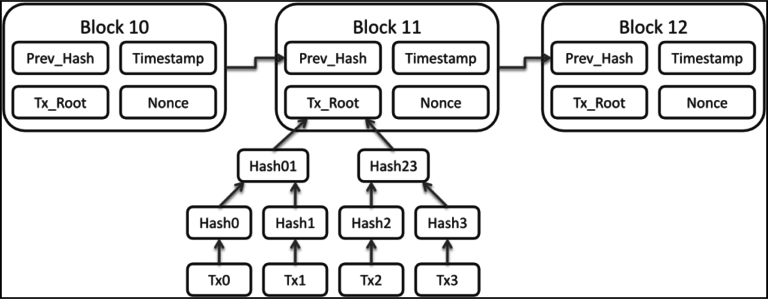
\includegraphics[width=0.9\textwidth]{blockHeader}
	\caption{Minh họa một blockheader}

\end{figure}

Một block header bao gồm:
\begin{itemize}
	\item Thời gian: timestamp hiện tại.
\item Độ khó bài toán.
\item Mã băm của block trước nó.
\item Nounce.
\item Mã băm của Merkle Root.
\end{itemize}

\chapter{Đồng thuận }

Blockchain là những hệ thống phân tán bao gồm những cá thể khác nhau hành động phụ thuộc vào động cơ 

Bất kể khi nào một giao dịch mới được đưa lện hệ thống mạng, các nút có thể lựa chọn hoặc thêm sao chép đó vào sổ cái của họ hoặc bỏ qua nó. Khi phần lớn các cá thể trong mạng đồng ý với một trạng thái (trong hai trạng thái trên),  sự đồng thuận đạt được.

Một vấn đề nền tảng trong các hệ thống điện toán phân toán và đa tác nhân là đạt được sự tin cậy tổng quát trong sự hiện diện của một số tiến trình bị lỗi. Điều này thường yêu cầu quy trình nhằm đồng thuận về một số giá trị dữ liệu cần trong quá trình tính toán.

Các quy trình này được được gọi là sự đồng thuận.

Để tạo ra một giao thức đồng thuận bảo mật,  nó phải chịu được lỗi (fault tolerant).

Để hiểu được giao thức đồng thuận trong blockchain, trước hết cần phải nói đến \textit{Bài Toán Hai Vị Tướng} (Two Generals Problem) và phiên bản mở rộng \textit{Byzantine Generals’ Problem} và thảo luận về \textit{Byzantine Fault Tolerance} trong hệ thống phân tán và phi tập trung để cuối cùng thảo luận mối liên quan của các vấn đề trên với blockchan.

\section{Bài Toán Hai Vị Tướng}

Bài toán này (lần đầu được đăng vào năm 1975 và có tên gọi trên vào năm 1978) mô tả một trường hợp khi hai vị tướng cùng tấn công một kẻ thù chung. Tướng 1 được xem như chỉ huy và tướng kia là người đi theo. Đội quân của mỗi vị tướng tự bản thân không thể đánh bại được quân đội kẻ thù, vì vậy họ cần phải phối hợp và tấn công cùng lúc. 

Để họ có thể liên lạc và quyết định thời điểm, Tướng 1 phải gửi một tin nhắn đi qua trại địch, trong đó cung cấp thời gian đợt tấn công cho Tướng 2. Vì vậy, có khả năng tin nhắn sẽ bị bắt được bởi kẻ địch và vì vậy tin nhắn sẽ không tới nơi. Điều đó sẽ dẫn đến việc Tướng 1 tấn công trong khi Tướng 2 và quân đội của ông ta đứng yên.

Ngay cả khi tin nhắn thứ nhất vượt qua được, Tướng 2 phải báo (acknowledge, ACK, tương tự như 3-way handshake của TCP) rằng ông ta đã nhận được tin nhắn, nên ông ta phả gửi một tin nhắn về, vì vậy lập lại trường hợp cũ khi tin nhắn có thể bị bắt. Điều này dẫn đến vô hạn số lần ACK và vì vậy các vị tướng không thể đạt được một sự đồng thuận.

Không có cách nào đảm bảo rằng yêu cầu thứ hai - mỗi vị tướng chắc chắn rằng bên kia đã đồng ý với kế hoạch tấn công. Cả hai vị tướng sẽ đều lo lắng rằng tin nhắn cuối cùng của họ có tới nơi hay không.

\begin{figure}[h]
	\centering
	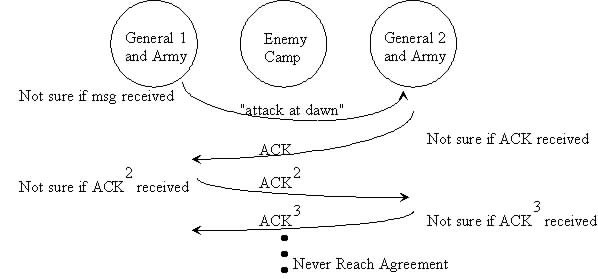
\includegraphics[width=0.9\textwidth]{twogeneral}
	\caption{Do xác suất tin nhắn không đi qua được luôn > 0, các tướng khong thể đạt được một sự đồng thuận với 100\% tin tưởng}
	
\end{figure}


Bài Toán Hai Vị Tướng đã được chứng minh là không thể giải.